\chapter{Background}
In this chapter, we introduce knowledge that is required to understand the content of this thesis.
We start with an introduction to processors in \Cref{sec:bg:cpu}.
In \Cref{sec:bg:compilers}, we overview how a compiler is typically implemented and which problems it has to solve that we want to tackle.
\Cref{sec:bg:compilers:backend} gives a more detailed introduction to compiler back-ends, which we aim to optimize in this thesis.
The compiler framework that we use as a basis is LLVM, which we introduce in \Cref{sec:bg:llvm}.
Eventually, we give a brief overview of the thesis's machine learning or data-driven approaches (\Cref{sec:bg:ml}).

% NOTE: Assume that the reader has common computer science knowledge!

% --- CPU ---
% Pipeline
% https://de.wikipedia.org/wiki/Pipeline_(Prozessor)
%   - Stages
%   - Hazards
% 
% Skalar - 1 in instruction per cycle possible
% Superskalar - more than 1 instruction per cycle possible
% https://de.wikipedia.org/wiki/Superskalarit%C3%A4t
%   - in order - static
%   - out of order - dynamic
%   - VLIW - multiple commands encoded into one long command

\section{Central Processing Unit}
\label{sec:bg:cpu}
Almost all computer systems use some \acp{cpu}.
It is the primary execution unit and executes the vast majority of computer programs on most systems.
It also handles access to other parts of the system.
These other parts can be the main memory, hard drives, network cards, or co-processors like a Graphics Processing Unit.

The \ac{cpu} executes mostly simple instructions, like add, subtract, multiply, shift, or load and store data to/from the main memory.
However, there are slightly more complex instructions on modern \acp{cpu} like combined multiply and add or cryptographic instructions.
The Instruction Set Architecture of a processor architecture defines all of the available instructions of a \ac{cpu}.

Most of the instructions do not have direct access to the main memory.
The instructions typically access data stored in the \ac{cpu} registers, which is the fastest memory available.
Hence, before we can execute instructions on some data, we must transfer this data to the registers.
We transfer the data back to the main memory once we finish our computations.
For example, if we want to compute 
\begin{equation}
    a=a\times a+b\times b+c\times c
    \label{eqn:bg:abc}
\end{equation}
we have to load the data from the variables $a$, $b$, and $c$, make the computations and store the result back to memory.
\Cref{tbl:bg:schedules} shows two possible example implementations in assembly language.
\Cref{fig:bg:example-dag} illustrates the dependencies between the \ac{cpu} instructions of the example implementations.

\begin{table}
    \begin{subtable}{.48\textwidth}\centering
        \begin{tabular}{rllcl} \toprule
            ID&\multicolumn{4}{c}{Instruction}\\
            \midrule
            $i_1$ & \iloccmd{load}{\ilocreg{arp}, @a}{\ilocreg{1}} \\
            $i_2$ & \iloccmd{load}{\ilocreg{arp}, @b}{\ilocreg{2}} \\
            $i_3$ & \iloccmd{load}{\ilocreg{arp}, @c}{\ilocreg{3}} \\
            $i_4$ & \iloccmd{mult}{\ilocreg{1}, \ilocreg{1}}{\ilocreg{1}} \\
            $i_5$ & \iloccmd{mult}{\ilocreg{2}, \ilocreg{2}}{\ilocreg{2}} \\
            $i_6$ & \iloccmd{mult}{\ilocreg{3}, \ilocreg{3}}{\ilocreg{3}} \\
            $i_7$ & \iloccmd{add}{\ilocreg{1}, \ilocreg{2}}{\ilocreg{1}} \\
            $i_8$ & \iloccmd{add}{\ilocreg{1}, \ilocreg{3}}{\ilocreg{1}} \\
            $i_9$ & \iloccmd{store}{\ilocreg{1}}{\ilocreg{arp}, @a} \\
            \bottomrule
        \end{tabular}
        \caption{}
        \label{tbl:bg:schedule-a}
    \end{subtable}
    \begin{subtable}{.48\textwidth}\centering
        \begin{tabular}{rllcl} \toprule
            ID&\multicolumn{4}{c}{Instruction}\\
            \midrule
            $i_1$ & \iloccmd{load}{\ilocreg{arp}, @a}{\ilocreg{1}} \\
            $i_4$ & \iloccmd{mult}{\ilocreg{1}, \ilocreg{1}}{\ilocreg{1}} \\
            $i_2$ & \iloccmd{load}{\ilocreg{arp}, @b}{\ilocreg{2}} \\
            $i_5$ & \iloccmd{mult}{\ilocreg{2}, \ilocreg{2}}{\ilocreg{2}} \\
            $i_3$ & \iloccmd{load}{\ilocreg{arp}, @c}{\ilocreg{3}} \\
            $i_6$ & \iloccmd{mult}{\ilocreg{3}, \ilocreg{3}}{\ilocreg{3}} \\
            $i_7$ & \iloccmd{add}{\ilocreg{1}, \ilocreg{2}}{\ilocreg{1}} \\
            $i_8$ & \iloccmd{add}{\ilocreg{1}, \ilocreg{3}}{\ilocreg{1}} \\
            $i_9$ & \iloccmd{store}{\ilocreg{1}}{\ilocreg{arp}, @a} \\
            \bottomrule
        \end{tabular}
        \caption{}
        \label{tbl:bg:schedule-b}
    \end{subtable}
    \caption[Example instruction schedules]{Example instruction schedules for \Cref{eqn:bg:abc}}
    \label{tbl:bg:schedules}
\end{table}

All the assembly code examples are written in the ILOC pseudo-code language~\cite{engineeringcompiler2007}.
Its instructions are of the form \iloccmdinl{instruction}{source}{target}.
The register \ilocreg{arp} is defined to point to the start of a memory block where all variables are stored.
Variables are addressed by adding an offset to the memory address in \ilocreg{arp}.
This is done by adding, \eg \iloc{@a} for the variable \iloc{a}.

Instructions that a \ac{cpu} executes are separated into different processing units.
Typical processing units on modern \acp{cpu} are arithmetic logical units, load/store units, floating-point units, or encryption units.
These units often exist redundantly on the \acp{cpu}.

\subsection{Classical Instruction Execution}
The execution of instructions works in multiple stages.
The stages depend on the specific implementation, \eg the ARM Cortex A53 has eight stages.
A typical example is four stages that usually exist in most \acp{cpu}.
These stages are:
\begin{enumerate}
    \item Fetch: 
        In this stage, the \ac{cpu} loads the instruction from memory, where the whole program is saved. 
    \item Decode:
        The operands of the instructions are determined.
        The actual memory address will be computed if there are memory addresses with offsets.
    \item Execution:
        Here, the instruction is executed with the given operands on the respective processing unit.
    \item Writeback:
        The computed result will be written back to the specified register during this stage.
\end{enumerate}

The \ac{cpu} executest one instruction at a time in this classical execution scheme.
It means that instructions can only start after all execution stages of the previous instruction have finished.
% Consequently, the throughput of instructions per cycle $t$ is always $t>1$, given that instructions require more than one cycle to execute.

\Cref{tbl:bg:pipeline} compares different execution models for the computation in \Cref{eqn:bg:abc}.
\Cref{tbl:bg:schedule-a} defines the used instruction schedule for this example.
In this example, we assume that each of the stages, Fetch (F), Decode (D), Execution (E), and Writeback (W), take a single \ac{cpu} cycle to finish.
\Cref{tbl:bg:wo-pipeline} shows the execution for this classical execution model.
We see that the execution takes 36 cycles to finish in this example.

\begin{table}
    % \scriptsize
    % \lstset{basicstyle=\ttfamily\scriptsize}
    \centering
    \parbox[b][0.8\textheight][s]{0.5\textwidth}{%
        \centering
        \subcaptionbox{CPU without pipeline\label{tbl:bg:wo-pipeline}}[0.48\textwidth]{%
            \scriptsize
            \begin{tabular}{rccccccccc} \toprule
                & \multicolumn{9}{c}{\fontsize{11pt}{9pt}\selectfont Instructions} \\
                \cmidrule{2-10}
                {\fontsize{11pt}{9pt}\selectfont CPU Cycle} & 
                {\fontsize{11pt}{9pt}\selectfont $i_1$} & 
                {\fontsize{11pt}{9pt}\selectfont $i_2$} & 
                {\fontsize{11pt}{9pt}\selectfont $i_3$} & 
                {\fontsize{11pt}{9pt}\selectfont $i_4$} & 
                {\fontsize{11pt}{9pt}\selectfont $i_5$} & 
                {\fontsize{11pt}{9pt}\selectfont $i_6$} & 
                {\fontsize{11pt}{9pt}\selectfont $i_7$} & 
                {\fontsize{11pt}{9pt}\selectfont $i_8$} & 
                {\fontsize{11pt}{9pt}\selectfont $i_9$} \\
                \midrule
                 1 & F &   &   &   &   &   &   &   &   \\ \rowcolor[gray]{.975}
                 2 & D &   &   &   &   &   &   &   &   \\
                 3 & E &   &   &   &   &   &   &   &   \\ \rowcolor[gray]{.975}
                 4 & W &   &   &   &   &   &   &   &   \\
                 5 &   & F &   &   &   &   &   &   &   \\ \rowcolor[gray]{.975}
                 6 &   & D &   &   &   &   &   &   &   \\
                 7 &   & E &   &   &   &   &   &   &   \\ \rowcolor[gray]{.975}
                 8 &   & W &   &   &   &   &   &   &   \\
                 9 &   &   & F &   &   &   &   &   &   \\ \rowcolor[gray]{.975}
                10 &   &   & D &   &   &   &   &   &   \\
                11 &   &   & E &   &   &   &   &   &   \\ \rowcolor[gray]{.975}
                12 &   &   & W &   &   &   &   &   &   \\
                13 &   &   &   & F &   &   &   &   &   \\ \rowcolor[gray]{.975}
                14 &   &   &   & D &   &   &   &   &   \\
                15 &   &   &   & E &   &   &   &   &   \\ \rowcolor[gray]{.975}
                16 &   &   &   & W &   &   &   &   &   \\
                17 &   &   &   &   & F &   &   &   &   \\ \rowcolor[gray]{.975}
                18 &   &   &   &   & D &   &   &   &   \\
                19 &   &   &   &   & E &   &   &   &   \\ \rowcolor[gray]{.975}
                20 &   &   &   &   & W &   &   &   &   \\
                21 &   &   &   &   &   & F &   &   &   \\ \rowcolor[gray]{.975}
                22 &   &   &   &   &   & D &   &   &   \\
                23 &   &   &   &   &   & E &   &   &   \\ \rowcolor[gray]{.975}
                24 &   &   &   &   &   & W &   &   &   \\
                25 &   &   &   &   &   &   & F &   &   \\ \rowcolor[gray]{.975}
                26 &   &   &   &   &   &   & D &   &   \\
                27 &   &   &   &   &   &   & E &   &   \\ \rowcolor[gray]{.975}
                28 &   &   &   &   &   &   & W &   &   \\
                29 &   &   &   &   &   &   &   & F &   \\ \rowcolor[gray]{.975}
                30 &   &   &   &   &   &   &   & D &   \\
                31 &   &   &   &   &   &   &   & E &   \\ \rowcolor[gray]{.975}
                32 &   &   &   &   &   &   &   & W &   \\
                33 &   &   &   &   &   &   &   &   & F \\ \rowcolor[gray]{.975}
                34 &   &   &   &   &   &   &   &   & D \\
                35 &   &   &   &   &   &   &   &   & E \\ \rowcolor[gray]{.975}
                36 &   &   &   &   &   &   &   &   & W \\
                \bottomrule
            \end{tabular}
            \vfill
        }
    }
    \hfill
    \parbox[b][0.8\textheight][s]{0.48\textwidth}{%
        \scriptsize
        \centering
        \subcaptionbox{CPU with scalar pipeline\label{tbl:bg:scalar-pipeline}}[0.48\textwidth]{%
            \begin{tabular}{rccccccccc} \toprule
                & \multicolumn{9}{c}{\fontsize{11pt}{9pt}\selectfont Instructions} \\
                \cmidrule{2-10}
                {\fontsize{11pt}{9pt}\selectfont CPU Cycle} & 
                {\fontsize{11pt}{9pt}\selectfont $i_1$} & 
                {\fontsize{11pt}{9pt}\selectfont $i_2$} & 
                {\fontsize{11pt}{9pt}\selectfont $i_3$} & 
                {\fontsize{11pt}{9pt}\selectfont $i_4$} & 
                {\fontsize{11pt}{9pt}\selectfont $i_5$} & 
                {\fontsize{11pt}{9pt}\selectfont $i_6$} & 
                {\fontsize{11pt}{9pt}\selectfont $i_7$} & 
                {\fontsize{11pt}{9pt}\selectfont $i_8$} & 
                {\fontsize{11pt}{9pt}\selectfont $i_9$} \\
                \midrule
                 1 & F &   &   &   &   &   &   &   &   \\ \rowcolor[gray]{.975}
                 2 & D & F &   &   &   &   &   &   &   \\
                 3 & E & D & F &   &   &   &   &   &   \\ \rowcolor[gray]{.975}
                 4 & W & E & D &   &   &   &   &   &   \\
                 5 &   & W & E & F &   &   &   &   &   \\ \rowcolor[gray]{.975}
                 6 &   &   & W & D & F &   &   &   &   \\
                 7 &   &   &   & E & D & F &   &   &   \\ \rowcolor[gray]{.975}
                 8 &   &   &   & W & E & D &   &   &   \\
                 9 &   &   &   &   & W & E &   &   &   \\ \rowcolor[gray]{.975}
                10 &   &   &   &   &   & W & F &   &   \\
                11 &   &   &   &   &   &   & D &   &   \\ \rowcolor[gray]{.975}
                12 &   &   &   &   &   &   & E &   &   \\
                13 &   &   &   &   &   &   & W &   &   \\ \rowcolor[gray]{.975}
                14 &   &   &   &   &   &   &   & F &   \\
                15 &   &   &   &   &   &   &   & D &   \\ \rowcolor[gray]{.975}
                16 &   &   &   &   &   &   &   & E &   \\
                17 &   &   &   &   &   &   &   & W &   \\ \rowcolor[gray]{.975}
                18 &   &   &   &   &   &   &   &   & F \\
                19 &   &   &   &   &   &   &   &   & D \\ \rowcolor[gray]{.975}
                20 &   &   &   &   &   &   &   &   & E \\
                21 &   &   &   &   &   &   &   &   & W \\
                \bottomrule
            \end{tabular}
        }
        \vfill
        \subcaptionbox{CPU with two-way superscalar in-order pipeline\label{tbl:bg:superscalar-pipeline}}[0.48\textwidth]{%
            \begin{tabular}{rccccccccc} \toprule
                & \multicolumn{9}{c}{\fontsize{11pt}{9pt}\selectfont Instructions} \\
                \cmidrule{2-10}
                {\fontsize{11pt}{9pt}\selectfont CPU Cycle} & 
                {\fontsize{11pt}{9pt}\selectfont $i_1$} & 
                {\fontsize{11pt}{9pt}\selectfont $i_2$} & 
                {\fontsize{11pt}{9pt}\selectfont $i_3$} & 
                {\fontsize{11pt}{9pt}\selectfont $i_4$} & 
                {\fontsize{11pt}{9pt}\selectfont $i_5$} & 
                {\fontsize{11pt}{9pt}\selectfont $i_6$} & 
                {\fontsize{11pt}{9pt}\selectfont $i_7$} & 
                {\fontsize{11pt}{9pt}\selectfont $i_8$} & 
                {\fontsize{11pt}{9pt}\selectfont $i_9$} \\
                \midrule
                 1 & F & F &   &   &   &   &   &   &   \\ \rowcolor[gray]{.975}
                 2 & D & D & F &   &   &   &   &   &   \\
                 3 & E & E & D &   &   &   &   &   &   \\ \rowcolor[gray]{.975}
                 4 & W & W & E &   &   &   &   &   &   \\
                 5 &   &   & W & F & F &   &   &   &   \\ \rowcolor[gray]{.975}
                 6 &   &   &   & D & D & F &   &   &   \\
                 7 &   &   &   & E & E & D &   &   &   \\ \rowcolor[gray]{.975}
                 8 &   &   &   & W & W & E &   &   &   \\
                 9 &   &   &   &   &   & W & F &   &   \\ \rowcolor[gray]{.975}
                10 &   &   &   &   &   &   & D &   &   \\
                11 &   &   &   &   &   &   & E &   &   \\ \rowcolor[gray]{.975}
                12 &   &   &   &   &   &   & W &   &   \\
                13 &   &   &   &   &   &   &   & F &   \\ \rowcolor[gray]{.975}
                14 &   &   &   &   &   &   &   & D &   \\
                15 &   &   &   &   &   &   &   & E &   \\ \rowcolor[gray]{.975}
                16 &   &   &   &   &   &   &   & W &   \\
                17 &   &   &   &   &   &   &   &   & F \\ \rowcolor[gray]{.975}
                18 &   &   &   &   &   &   &   &   & D \\
                19 &   &   &   &   &   &   &   &   & E \\ \rowcolor[gray]{.975}
                20 &   &   &   &   &   &   &   &   & W \\ 
                \bottomrule
            \end{tabular}
        }
    }
    \caption[Comparison of CPU pipeline implementations]{Comparison of CPU pipeline implementations for the example in \Cref{eqn:bg:abc}. 
    The used instruction schedule is defined in \Cref{tbl:bg:schedule-a}.}
    \label{tbl:bg:pipeline}
\end{table}

It is easy to see that the \ac{cpu} does not fully utilize all stages.
Only one stage is working at a time, and the rest of the stages are doing nothing for the most time.
This behavior is ineffective and addressed by the following execution model.

\subsection{Scalar Pipeline Execution}
This execution model uses the fact that most stages are waiting most of the time.
The improvement is that now, one execution can be scheduled in every \ac{cpu} cycle.

See in \Cref{tbl:bg:scalar-pipeline} that this change introduces parallelism, and the \ac{cpu} executes the first three instructions concurrently.
The theoretically best case is that all the stages are working in every cycle and are never waiting.
This is not always possible, as we can see in the example.
We cannot start instruction $i_4$ (\iloccmdinl{mult}{\ilocreg{1},~\ilocreg{1}}{\ilocreg{1}}) in the fourth \ac{cpu} cycle, because we have a dependency on the result of instruction $i_1$ (\iloccmdinl{load}{\ilocreg{arp},~@a}{\ilocreg{1}}).
In the fifth cycle, the result of instruction $i_1$ was written back and we can start instruction $i_4$.
Different reasons of hazards exist that cause these bubbles in the pipeline.
\begin{itemize}
    \item Resource Hazards:
        When the \ac{cpu} needs to access a resource, which is already accessed and thus blocked, the access cannot happen and has to wait.
        This could, for example, happen with registers that have only one access line.
        Redundancy of hardware units can solve or mitigate this problem.
    \item Data Hazards:
        Three types of different data hazards exist when two instructions want to access the same register:
        \begin{itemize}
            \item Read after write: A instruction has to wait until a previous instruction has produced the result that the latter has to read.
            \item Write after read: A instruction has to wait until a previous instruction has read a register, that the latter has to overwrite.
            \item Write after write: A instruction has to wait until a previous instruction has written a register, that the latter wants to write to, too.
        \end{itemize}
        These hazards are typically solved by sorting the instructions or waiting and introducing bubbles into the pipeline when it is unavoidable.
    \item Control Hazards:
        It is not always obvious which instruction should be executed next due to if/else constructs or loops.
        Usually, the \ac{cpu} will execute one branch speculatively and abort the instructions if it is the wrong branch.
        This problem is typically approached by branch prediction mechanisms that can be done in the compiler and on the hardware.
\end{itemize}

\subsection{Superscalar Pipeline Execution}
\label{sec:bg:superscalar-cpu}
The next progression from the scalar pipeline is this pipeline model.
The difference is that we can start multiple instructions in the same \ac{cpu} cycle.
Consequently, this increases the level of parallelism.
The number of instructions that can start simultaneously depends on the specific hardware. % A53 2-way

\Cref{tbl:bg:superscalar-pipeline} shows an example execution of a two-way superscalar pipeline.
This is especially interesting to compare with the scalar pipeline in \Cref{tbl:bg:scalar-pipeline}.
Note that now, instructions 1 and 2 are scheduled in the same \ac{cpu} cycle.
If we had simulated a three-way superscalar pipeline, we could have started instructions 1-3 in the first cycle.
However, we still have a runtime improvement of one cycle compared to the scalar pipeline.

Various ways exist to implement superscalar pipelines.
The three most typical implementations are:
\begin{itemize}
    \item In order (static): 
        These type of \acp{cpu} take the instructions as they come and check if they can be executed simultaneously.
        The compiler defines the instruction schedule.
    \item Out-of-order (dynamic): 
        Dynamic superscalar CPUs can see the following n instructions and reschedule them to achieve higher parallelism.
        This means that the compiler does not fully control the executed instruction schedule, which is essential for this thesis.
    \item Very Long Instruction Word: 
        The compiler can define which instructions the CPU will execute simultaneously for this type of superscalar pipeline.
        This assignment works by wrapping multiple instructions into a single instruction, thus the name.
\end{itemize}

\subsection{Instruction Schedules}
\label{sec:bg:cpu-schedule}
Looking at \Cref{fig:bg:example-dag}, we see that the dependencies allow different instruction schedules.
For example, we could use a breadth-first approach and execute all the load instructions first, then all the multiplications, et cetera.
On the contrary, we could use a depth-first approach and execute the load and multiplication for variable a, then for b, et cetera.
These two schedules are defined in \Cref{tbl:bg:schedules} and compared in this section.

With the classical execution scheme with no pipeline, the instructions schedule is irrelevant for the runtime
However, the runtime improvements that \acp{cpu} gain by pipelines depend heavily on the instruction schedule.
We demonstrate this on two instruction schedules that we defined in \Cref{tbl:bg:schedules}.

We illustrate the execution of the two schedules in \Cref{tbl:bg:schedule-comparison}.
This example assumes that load and store instruction need three cycles to finish, multiplications need two cycles and add instruction need one cycle.
Here, we ignore the phases of the instruction execution for simplicity.
We demonstrate the execution of a two-way superscalar in-order processor.
The goal here is to have an instruction schedule that allows maximum parallelism.
\begin{table}
    \scriptsize
    \begin{subtable}{0.48\textwidth}
        \begin{tabular}{rccccccccc} \toprule
            & \multicolumn{9}{c}{\fontsize{11pt}{9pt}\selectfont Instructions} \\
            \cmidrule{2-10}
            {\fontsize{11pt}{9pt}\selectfont CPU Cycle} & 
            {\fontsize{11pt}{9pt}\selectfont $i_1$} & 
            {\fontsize{11pt}{9pt}\selectfont $i_2$} & 
            {\fontsize{11pt}{9pt}\selectfont $i_3$} & 
            {\fontsize{11pt}{9pt}\selectfont $i_4$} & 
            {\fontsize{11pt}{9pt}\selectfont $i_5$} & 
            {\fontsize{11pt}{9pt}\selectfont $i_6$} & 
            {\fontsize{11pt}{9pt}\selectfont $i_7$} & 
            {\fontsize{11pt}{9pt}\selectfont $i_8$} & 
            {\fontsize{11pt}{9pt}\selectfont $i_9$} \\
            \midrule
             1 & X & X &   &   &   &   &   &   &   \\ \rowcolor[gray]{.975}
             2 & X & X & X &   &   &   &   &   &   \\
             3 & X & X & X &   &   &   &   &   &   \\ \rowcolor[gray]{.975}
             4 &   &   & X & X & X &   &   &   &   \\
             5 &   &   &   & X & X & X &   &   &   \\ \rowcolor[gray]{.975}
             6 &   &   &   &   &   & X & X &   &   \\
             7 &   &   &   &   &   &   &   & X &   \\ \rowcolor[gray]{.975}
             8 &   &   &   &   &   &   &   &   & X \\
             9 &   &   &   &   &   &   &   &   & X \\ \rowcolor[gray]{.975}
            10 &   &   &   &   &   &   &   &   & X \\
            \bottomrule
        \end{tabular}
        \caption{Execution of instruction schedule from \Cref{tbl:bg:schedule-a}}
        \label{tbl:bg:schedule-comparison-a}
    \end{subtable}
    \hfill
    \begin{subtable}{0.48\textwidth}
        \begin{tabular}{rccccccccc} \toprule
            & \multicolumn{9}{c}{\fontsize{11pt}{9pt}\selectfont Instructions} \\
            \cmidrule{2-10}
            {\fontsize{11pt}{9pt}\selectfont CPU Cycle} & 
            {\fontsize{11pt}{9pt}\selectfont $i_1$} & 
            {\fontsize{11pt}{9pt}\selectfont $i_4$} & 
            {\fontsize{11pt}{9pt}\selectfont $i_2$} & 
            {\fontsize{11pt}{9pt}\selectfont $i_5$} & 
            {\fontsize{11pt}{9pt}\selectfont $i_3$} & 
            {\fontsize{11pt}{9pt}\selectfont $i_6$} & 
            {\fontsize{11pt}{9pt}\selectfont $i_7$} & 
            {\fontsize{11pt}{9pt}\selectfont $i_8$} & 
            {\fontsize{11pt}{9pt}\selectfont $i_9$} \\
            \midrule
             1 & X &   &   &   &   &   &   &   &   \\ \rowcolor[gray]{.975}
             2 & X &   &   &   &   &   &   &   &   \\
             3 & X &   &   &   &   &   &   &   &   \\ \rowcolor[gray]{.975}
             4 &   & X & X &   &   &   &   &   &   \\
             5 &   & X & X &   &   &   &   &   &   \\ \rowcolor[gray]{.975}
             6 &   &   & X &   &   &   &   &   &   \\
             7 &   &   &   & X & X &   &   &   &   \\ \rowcolor[gray]{.975}
             8 &   &   &   & X & X &   &   &   &   \\
             9 &   &   &   &   & X &   &   &   &   \\ \rowcolor[gray]{.975}
            10 &   &   &   &   &   & X & X &   &   \\
            11 &   &   &   &   &   & X &   &   &   \\ \rowcolor[gray]{.975}
            12 &   &   &   &   &   &   &   & X &   \\
            13 &   &   &   &   &   &   &   &   & X \\ \rowcolor[gray]{.975}
            14 &   &   &   &   &   &   &   &   & X \\
            15 &   &   &   &   &   &   &   &   & X \\
            \bottomrule
        \end{tabular}
        \caption{Execution of instruction schedule from \Cref{tbl:bg:schedule-b}}
        \label{tbl:bg:schedule-comparison-b}
    \end{subtable}
    \caption[Schedule comparison on a two-way superscalar in-order architecture]{Execution of the instruction schedules \Cref{tbl:bg:schedule-a} and \Cref{tbl:bg:schedule-b} on a two-way superscalar in-order architecture. 
    We assume that load and store instructions require three cycles, multiplies two cycles and adds one cycle.}
    \label{tbl:bg:schedule-comparison}
\end{table}

We achieve parallel execution in \Cref{tbl:bg:schedule-comparison-a} for the instructions $i_1$ and $i_2$ and $i_4$ and $i_5$.
We cannot schedule the instructions $i_3$ and $i_4$ together because $i_4$ has to wait for $i_1$ to finish.

In the execution in \Cref{tbl:bg:schedule-comparison-b}, we can schedule the instructions $i_4$ and $i_2$, $i_5$ and $i_3$, and $i_6$ and $i_7$ together in pairs of two.
However, the overall execution is with 15 cycles slower than the 10 cycles of the execution in \Cref{tbl:bg:schedule-comparison-a}.

Instruction scheduling is not a trivial task, and much research was published to optimize this problem.
However, the more complicated \acp{cpu} become, the harder it gets to generate fast instruction schedules.

\section{Compilers}
\label{sec:bg:compilers}
A compiler is a tool that helps make programs, written in a high-level language, executable on a specific machine.
The compilers' goal is to translate from a high-level language to a low-level language or machine code.
During the translation, the compiler ensures that the output program is a correct representation of the input.
Further, compilers typically aim to optimize the source program with a defined goal, \eg runtime performance or memory usage.

Making a high-level language program executable includes more tasks than the translation, which is a non-trivial task.
For example, other steps include linking the program with libraries, especially standard libraries, that implement basic functionalities.
Next, it has to be prepared to interact with a runtime library.
These topics are out of the scope of this thesis, and we do not discuss them further.

The implementation of a compiler is typically separated into three phases which apply modifications to the given code with a defined output format.
\begin{enumerate}
    \item The compiler transforms from the high-level language to an \ac{ir} in the front-end phase.
    \item The compiler applies optimizations on the \ac{ir} and outputs the code in the same format.
    \item In the back-end phase, the compiler transforms the \ac{ir} to assembly code or machine code.
\end{enumerate}
We explain these three phases in more detail, especially the back-end phase, which we are working on in this thesis.

\subsubsection{Basic Block}
Compilers typically perform their transformations on a per basic block level.
This includes the instruction scheduling in the back-end phase (see \Cref{sec:bg:compilers:backend}).

A basic block is a sequential collection of instructions.
They have a single defined starting instruction and a single defined ending instruction.
That means, once a basic block executes, all its instructions execute.
Consequently, basic blocks cannot contain branches.
However, function calls are allowed since they return to the next instruction after the call and continue their execution.

\subsection{Front-End}
\label{sec:bg:compilers:frontend}
The front-end phase is the first step in the translation process.
Its implementation is dependent on the source language that has to be translated.
A typical front-end includes a scanner, a syntax checker/parser, a context-sensitive analysis, and translation into an \ac{ir}.
The scanner translates a character stream into a token stream.
The parser then takes these tokens and is checked against the grammar defined by the source language.
Even with a syntactically correct program, there can still be errors in the code, \eg assignments of incompatible types.
These are checked during the context-sensitive analysis phase.
Eventually, the source code is translated into a \ac{ir} which will be used as input to the optimizer and the back-end.
The \ac{ir} is compiler-dependent and typically defined as a \ac{ssa} form.

There might be additional steps required depending on the source language.
C/C++ compilers, for example, use a preprocessor to replace macros like \lstinline{#include} and \lstinline{#define} with their actual values.

\subsection{Optimizer}
\label{sec:bg:compilers:optimizer}
The usage of an \ac{ir} abstracts away the source language and the target hardware and permits applying more standardized passes in the compilation process.
These additional passes transform \ac{ir} to \ac{ir}.
Note that this step is optional and not required to produce correct translations.
This step aims to optimize the code for more efficient execution in a source- and target-independent manner.
Efficient can mean different things here.
The transformed code might produce, \eg a faster program, a smaller program, or a program with less power consumption.

There exist a large number of optimization passes in most compilers.
They range from relatively simple optimizations, like replacing constant variables with their actual value, to more advanced ones that might, for example, simplify computations with the rules of algebra.

\subsection{Back-end}
\label{sec:bg:compilers:backend}
The overall goal of the compiler's back-end is to transform the \ac{ir} to code for the target hardware.
Further, it also decides where the processor saves variables (registers only or memory) and, thus, how they will be accessed.
We explain the necessary steps in more detail.

\subsubsection{Instruction Selection}
First, the compiler translates the input \ac{ir} representation.
As the \ac{ir} is already in \ac{ssa} form, the translation step mostly maps \ac{ir} instructions to instructions defined in the Instruction Set Architecture of the target hardware.
The instruction selection is not a one-to-one mapping in all cases, but sometimes, \ac{ir} instructions are represented by multiple hardware instructions.

Note that the compiler chooses actual processor instructions, but registers are not assigned yet.
Variables are assigned to an unlimited number of virtual registers.
This means that the compiler still works in an \ac{ssa} form regarding the registers.

\subsubsection{Instruction Scheduling}
In the instruction scheduling phase, the compiler tries to generate an optimal ordering over the instructions of a basic block.
Optimal in this context usually means to optimize for short runtimes.

% Mixed: why important
We have seen how different schedules influence the runtime performance in \Cref{tbl:bg:schedule-comparison}.
The objective of this thesis is to optimize this instruction scheduling step in the compiler back-end.
Here we explain how instruction scheduling typically works.

% Why important - but rewrite this probably
As stated in \Cref{sec:bg:cpu-schedule}, different types of \ac{cpu} pipelines are influenced by the instruction schedule.
When we look at the superscalar pipelines (see \Cref{sec:bg:superscalar-cpu}), the out-of-order pipeline will benefit the least from better instruction schedules because it can reschedule the instructions themselves.
The other two superscalar pipelines benefit more from better instruction schedules because they might stall completely until a hazard is cleared.
However, all pipelined execution models might benefit from better instruction schedules.

% Why hard
Instruction scheduling is a challenging problem.
One reason for that is that it is NP-complete to find an optimal schedule.
It is necessary to work with heuristics and generate approximations to optimal schedules.
Additionally, processors get more and more optimized in special cases.
That makes them faster, but it also becomes harder to predict what they will do in a given situation, \ie to predict how long it will take to execute a given instruction.
Optimizations that have an influence on this are hardware branch prediction, pipeline forwarding, hardware interlocks, or early exits.
This are only a few examples and not a complete list.
Therefore, the problem is not only NP-complete, but also has to be solved with unreliable data.

% How
Like the transformations in the optimizer stage, the instruction scheduling is typically done on a basic block level.
However, there exists research on extending the scope of instruction scheduling.
\todo{Add references, see book}

Compilers typically use the list scheduling approach to find an approximately optimal solution.
List scheduling is more of a framework than a specific algorithm.
We will explain here how it works in general.

% How
The compiler typically transforms the sequence of instructions into a dependency graph to analyze a given basic block.
The dependency graph defines which instructions need to be scheduled before a given instruction can be scheduled.
The nodes in the dependency graph represent an instruction, and the edges represent dependencies.
The edges point from a given instruction to all the instructions on which it depends.
Dependency graphs are modeled as \acp{dag}, and the valid schedules are defined as the set of the valid traversals for the given \ac{dag}.

% How
In \Cref{fig:bg:example-dag} we see that before we can execute the \iloc{store} ($i_9$) instruction to move the result back to memory, we have to run the last \iloc{add} ($i_8$) instruction.
This \iloc{add} ($i_8$) instruction depends on another \iloc{add} ($i_7$) and a \iloc{mult} ($i_6$) instruction.
The nodes that have no outgoing edge are leafs ($i_1$, $i_2$, and $i_3$) and can be scheduled directly in the beginning without any constraint.
\begin{figure}
    \centering

    % TODO: move these definitions somewhere else?
    \definecolor{darkgray}{HTML}{3D4752}
    \tikzstyle{instr} = [rectangle, rounded corners, minimum width=3cm, minimum height=1cm,text centered]%, text=white, fill=darkgray]
    \tikzstyle{arrow} = [thick,->,>=stealth]
    \begin{tikzpicture}[node distance=2cm]
        \node (load_a) [instr] {$i_1$: \lstinline{load @a}};
        \node (mul_a_a) [instr, below of=load_a] {$i_4$: \lstinline{mult}};
        \node (load_b) [instr, right of=load_a, xshift=3cm] {$i_2$: \lstinline{load @b}};
        \node (mul_b_b) [instr, below of=load_b] {$i_5$: \lstinline{mult}};
        \node (load_c) [instr, right of=load_b, xshift=3cm] {$i_3$: \lstinline{load @c}};
        \node (mul_c_c) [instr, below of=load_c] {$i_6$: \lstinline{mult}};
        \node (add_a_b) [instr, below of=mul_b_b] {$i_7$: \lstinline{add}};
        \node (add_ab_c) [instr, below of=add_a_b] {$i_8$: \lstinline{add}};
        \node (store) [instr, below of=add_ab_c] {$i_9$: \lstinline{store @a}};
        
        \draw [arrow] (mul_a_a) -- (load_a);
        \draw [arrow] (mul_b_b) -- (load_b);
        \draw [arrow] (mul_c_c) -- (load_c);
        \draw [arrow] (add_a_b) -- (mul_a_a);
        \draw [arrow] (add_a_b) -- (mul_b_b);
        \draw [arrow] (add_ab_c) -- (add_a_b);
        \draw [arrow] (add_ab_c) -- (mul_c_c);
        \draw [arrow] (store) -- (add_ab_c);    
    \end{tikzpicture}
    \caption[Dependency Graph]{Dependency graph for the example in \Cref{eqn:bg:abc}.}
    \label{fig:bg:example-dag}
\end{figure}

Next, the compiler assigns priority scores to each node.
Different scores could analyze the instruction runtime or the cumulated runtime from the instruction to the next leaf.
A goal is often to reduce the register pressure. 
We explain this in the Register Allocation phase.
Multiple scores can be assigned to break ties between instructions.

Eventually, the compiler collects the instructions that are ready to schedule.
In the beginning, that are the leafs of the \ac{dag}.
In the example in \Cref{fig:bg:example-dag} those are the instructions $i_1$, $i_2$, and $i_3$.
It schedules one of these instructions.
This process is repeated until all instructions are scheduled.
If the compiler chooses to schedule instruction $i_1$ first, then the instructions available in the next round are $i_2$, $i_3$, and $i_4$.
The described method is a top-down approach, but it is equally solvable in a bottom-up fashion.

% How
% Is this true? Probably still works with cycles internally.
% For modern processors the compiler just has to define a sorting of instructions.
% However, on older processors, it was necessary to define the cycle in which a instruction would start.
% In the case of processor stalls, the compiler would have to insert \iloc{nop} (no operation) instructions which just do nothing for one cycle.
% Modern processors have hardware interlocks which cause the processor to wait until all hazards are cleared. % https://en.wikipedia.org/wiki/Interlock_(engineering)



\subsubsection{Register Allocation}
In the previous instruction scheduling phase, the compiler still works with an infinite amount of virtual registers.
The processors have a defined set of different classes registers, \eg different registers often exist for integer and floating-point numbers.
In this phase, the compiler's goal is to map $n$ virtual registers to $m$ hardware registers, where $m$ is typically a lot smaller than $n$.

Registers are the fastest memory type in computers to access data.
It is often the only way to access data directly, \ie data must be transferred from main memory to registers and vice versa by load and store instructions.
Due to its speed, registers are also costly and thus available in a limited number.

The mapping to hardware registers is not always possible. 
In that case, memory spills are introduced.
This means that the content of some registers has to be outsourced to memory.
So, an additional store instruction to move the data to memory and an additional load instruction must be added to the code to get the data back into a register when it is needed.
These spills are costly for the runtime performance, and the goal is to reduce them.

Like instruction scheduling, register allocation is also a challenging problem.
It can be reduced to the graph coloring problem, which is NP-complete.

The runtime performance impact of the register allocation is also highly interdependent with the instruction scheduling~\cite{goodman1988code}.
Instruction schedules can be optimized for reducing the number of live variables.
The instruction schedules in \Cref{tbl:bg:schedules} both use the three registers \ilocreg{1}, \ilocreg{2}, and \ilocreg{3}.
However, the instruction schedule in \Cref{tbl:bg:schedule-reduced-regs} only uses the two registers \ilocreg{1}, and \ilocreg{2}.
The variable \iloc{b} is not used after instruction $i_7$, so its register \ilocreg{2} can be reused for variable \iloc{c}.
It does not mean that this is always faster,\eg thus it is not always helpful to optimize for reduced register pressure when there are enough registers to prevent spills.

\begin{table}
    \centering
    \begin{tabular}{rllcl} \toprule
        ID&\multicolumn{4}{c}{Instruction}\\
        \midrule
        $i_1$ & \iloccmd{load}{\ilocreg{arp}, @a}{\ilocreg{1}} \\
        $i_2$ & \iloccmd{load}{\ilocreg{arp}, @b}{\ilocreg{2}} \\
        $i_4$ & \iloccmd{mult}{\ilocreg{1}, \ilocreg{1}}{\ilocreg{1}} \\
        $i_5$ & \iloccmd{mult}{\ilocreg{2}, \ilocreg{2}}{\ilocreg{2}} \\
        $i_7$ & \iloccmd{add}{\ilocreg{1}, \ilocreg{2}}{\ilocreg{1}} \\
        $i_3$ & \iloccmd{load}{\ilocreg{arp}, @c}{\ilocreg{2}} \\
        $i_6$ & \iloccmd{mult}{\ilocreg{2}, \ilocreg{2}}{\ilocreg{2}} \\
        $i_8$ & \iloccmd{add}{\ilocreg{1}, \ilocreg{2}}{\ilocreg{1}} \\
        $i_9$ & \iloccmd{store}{\ilocreg{1}}{\ilocreg{arp}, @a} \\
        \bottomrule
    \end{tabular}
    \caption{Instruction schedule with reduced register pressure}
    \label{tbl:bg:schedule-reduced-regs}
\end{table}

\section{LLVM Compiler Infrastructure}
\label{sec:bg:llvm}
LLVM~\cite{LLVM:CGO04} is an open-source framework for compiler technology.
It started as a research project in 2000 and is nowadays widely used in compilers for various languages.
It is most known as the back-end of the C/C++ compiler \iloc{clang}, but is also used for the languages Rust (\iloc{rustc}), Go (\iloc{gollvm}), and more.

The LLVM framework framework is easily extendable.
This is especially true for new source languages and target hardwares.
Additionally, also details can be added to the compiler easily, like optimizations passes or instruction schedulers.

We choose to work with the LLVM framework because it gives us full control over the compilation process.
It is easy to add new instruction schedulers and implement transformation passes for the LLVM \ac{ir}.

The LLVM project was designed to make the three compiler phases executable in isolation.
That means we can run an LLVM front-end like \iloc{clang}, or \iloc{rustc} to generate LLVM \ac{ir} code.
From there, the optimizer program \iloc{opt} can modify the LLVM \ac{ir} code.
This step is independent of the source language and the target hardware.
Eventually, we can translate the LLVM \ac{ir} into object or assembly code by calling the LLVM back-end \iloc{llc} and configure it to use our custom instruction scheduler.

% \subsection{Intermediate Representation}
\subsection{Directed Acyclic Graph}
As explained in \Cref{sec:bg:compilers:backend}, LLVM also uses a \ac{dag} representation for basic blocks internally.
The C++ class \lstinline|SelectionDAG| defines the LLVM \ac{dag}.
LLVM comes with functionality to plot their internal \acp{dag}.
\Cref{fig:bg:llvm-dag} shows an example.
\begin{figure}
    \centering
    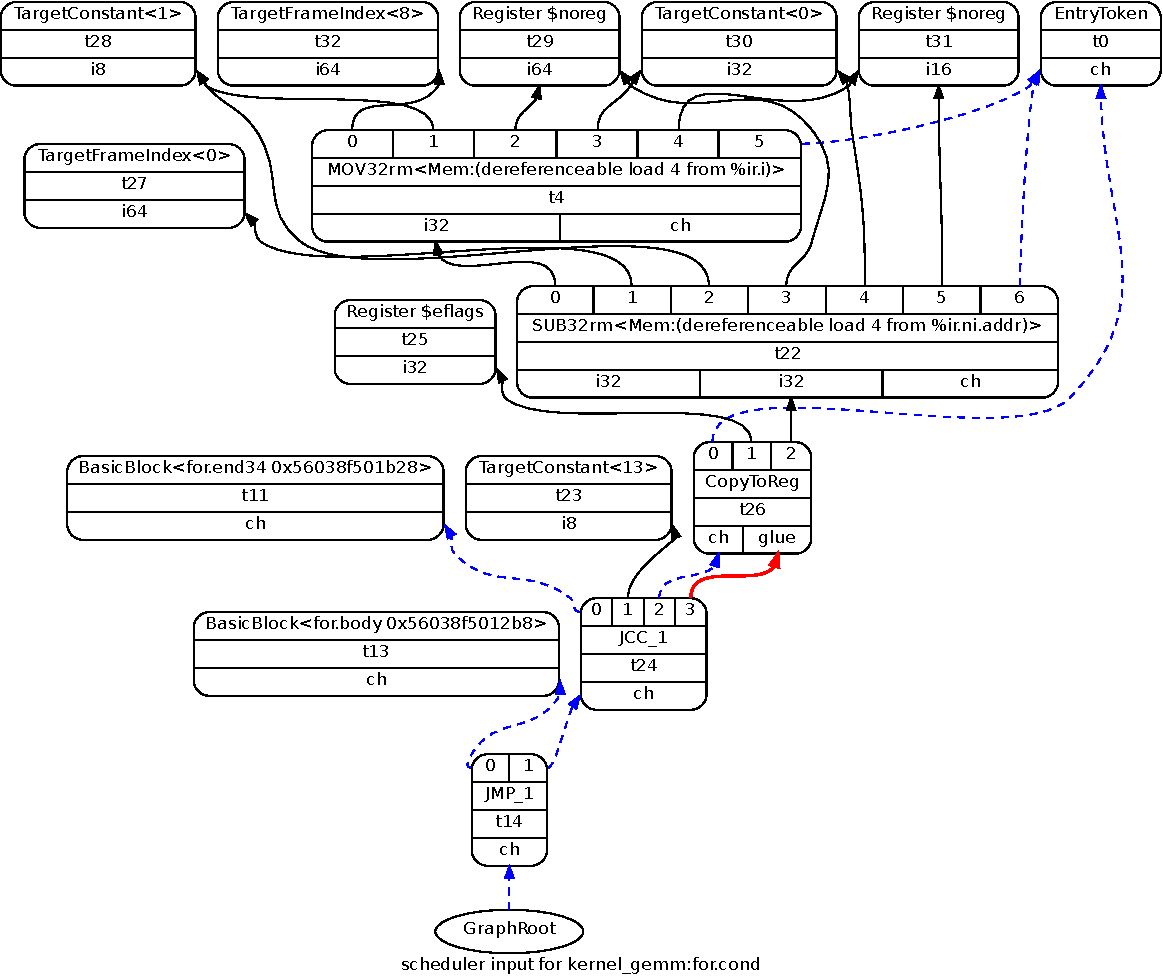
\includegraphics[width=\textwidth]{img/example-dag-crop.pdf}
    \caption[Example \aclu{dag} generated by LLVM]{Example \ac{dag} generated by LLVM. It shows the (AArch64) instructions defined by LLVM and the dependencies between the instructions.}
    \label{fig:bg:llvm-dag}
\end{figure}

Arrowed edges represent the dependencies between instructions.
The arrows point from a given instruction to one of its dependency instructions.
Three different types of edges exist that represent different types of dependencies:
\begin{itemize}
    \item Black: Represents a data flow dependency. That means that an instruction consumes the result of the previous instruction.
    \item Dashed Blue: This edge ensures that two unrelated instructions in terms of data flow remain scheduled in the correct order.
        In \Cref{fig:bg:llvm-dag}, the conditional jump instruction \lstinline|t24| must be scheduled before the unconditional jump instruction \lstinline|t14|, even though there is no data-flow dependency between these two.
    \item Red: This edge represents two instructions that must be scheduled together without any instructions between them.
\end{itemize}

The nodes in the LLVM \ac{dag} represent instructions.
Outgoing dependencies are numbered and placed in the top row.
If no dependencies exist, this row is missing.
The instruction name is written in the next node row, which is the top row if there are no outgoing dependency edges.
The next row shows an internally used instruction ID.
The generated output type of this instruction is placed in the bottom row. 
There are three possible values for the output type:
\begin{itemize}
    \item The datatype of the instructions result, \eg \lstinline|i32|, \lstinline|i64|, \lstinline|f32|, \lstinline|f64|, or \lstinline|v2f32|.
    \item \lstinline|ch|, which represents no data but is placed together with the dashed blue dependencies.
    \item \lstinline|glue| also does not represent any data but is placed together with the red dependencies.
\end{itemize}

Even though the instruction scheduling has already finished, there can still be LLVM pseudo instructions.
They get resolved in later stages.
The LLVM \ac{dag} always contains an \lstinline|EntryToken| pseudo instruction which gets always scheduled first.
Additionally, there is the \lstinline|GraphRoot| node at the bottom does not represent any instruction and will not get scheduled.
The \lstinline|BasicBlock| pseudo instructions represent the \lstinline|EntryToken| of another basic block.

\subsection{Instruction Scheduling}
The instruction scheduling happens in two phases in LLVM.
There is an instruction scheduling phase before register allocation (pre-RA) and after register allocation (post-RA).
LLVM makes the main scheduling decisions in the pre-RA phase.
The post-RA phase is only there to eliminate some small inefficiencies that can be detected, once the hardware registers are assigned.
When we speak of instruction scheduling in the context of LLVM, we mean the pre-RA phase from here on.

The maintainers of the LLVM framework are working on replacing the current pre-RA scheduling classes.
The new schedulers use the \lstinline|MIScheduler| class as their base.
Initially, instruction scheduling was integrated in the code of the instruction selection phase and worked on the \lstinline|ScheduleDAG| class.
We decided to base our work on the older implementation as it is still wider spread, and most production-used instruction schedulers are implemented in this manner.

There are already different instruction scheduler implementations that come with LLVM.
These can be used by configuring the \lstinline|llc| back-end with the command line option \lstinline|--pre-RA-sched=| and the possible choices:
\begin{itemize}
    \item \lstinline|vliw-td|: Scheduler for VLIW processors
    \item \lstinline|list-ilp|: List scheduler for balancing instruction-level parallelism and register pressure
    \item \lstinline|list-hybrid|: List scheduler for balancing latency and register pressure
    \item \lstinline|list-burr|: List scheduler for reducing register usage
    \item \lstinline|source|: Similar to \lstinline|list-burr|, but prefers the ordering from LLVM \ac{ir}
    \item \lstinline|linearize|: Does not schedule but returns instructions as they come in from LLVM \ac{ir}
    \item \lstinline|fast|: For compile-time optimized suboptimal scheduler
    \item \lstinline|default|: The best scheduler for the used target hardware
\end{itemize}
We use the \lstinline|default| scheduler as our baseline in all experiments.


\section{Data-Driven Methods}
\label{sec:bg:ml}
Throughout this thesis, we utilize data-driven methods for different tasks.
We use Monte Carlo Tree Search for finding good instruction schedules and build a dataset.
We describe this method in \Cref{sec:bg:mcts}.
For learning how to generate good schedules for unseen basic blocks, we use Support Vector Machines and Neural Networks, which we explain in \Cref{sec:bg:svm} and \Cref{sec:bg:nn}.

\subsection{Monte Carlo Tree Search}
\label{sec:bg:mcts}
\ac{mcts}~\cite{abramson1990expected} is a randomized search method to search optimal decisions.
When a computer's task is to play a board game, it has to make decisions, and from previous decisions, it has to make new decisions.
This process continues until the game is over.
From the beginning of the game until the end, we can model the decision-making process as a decision tree.
For small games, like Tic Tac Toe, it is possible to use the trivial Minimax algorithm, which will check all possible paths in the decision tree.
However, for games like Chess, there are too many possible paths for a computer to simulate.
The same is true for our instruction scheduling problem.
Every path in the decision tree represents an instruction schedule, which has to be compiled and executed to evaluate it.
This process is too slow for the number of possible instruction schedules that exist for a typical basic block.

\ac{mcts} works by exploring one level of decisions  and finishing the path with random decisions.
When all decisions in a level were seen at least once, the algorithm will balance exploitation and exploration, which means it chooses the best possible decision most of the time.
However, sometimes it will choose another decision to learn more in an undiscovered part of the decision tree.
This balancing causes \ac{mcts} to learn how to extend the paths with better decisions.

We will explain the algorithm in more detail here.
The \ac{mcts} algorithm consists of four steps.
These are:
\begin{enumerate}
    \item Selection Phase:
        The algorithm starts from the root node of the \ac{mcts} tree and iterates down through the nodes by applying a child selection policy.
        It stops when it finds a node that has children, but not all children where visited yet.
        These nodes are called expandable nodes.
    \item Expansion Phase:
        The \ac{mcts} tree gets expanded by adding the available children to the selected node from the previous step.
        The new children are created with a view count of 0.
    \item Simulation Phase:
        From the selected node, the path through the \ac{mcts} tree will be filled with randomly chosen nodes until a terminal state is reached.
        In this phase, no nodes will be added to the tree.
        They will just be used to fill the path.
        This path through the \ac{mcts} tree gets evaluated, \eg by playing the board game with the decisions or in our case by checking the runtime of the instruction schedule.
    \item Backpropagation Phase:
        The evaluation of that path gets applied to the statistics of all the nodes from the path present in the \ac{mcts} tree.
\end{enumerate}
The node statistics are typically just two values.
First, the count of how many times a node was included in a simulation.
The second value is the cumulated evaluation metric.
Typically, cumulated means the average value.
However, in our case, it is beneficial to use the maximum value instead of the average.
This was also mentioned in~\cite{bjornsson2009cadiaplayer} and generalized for single-player games.

The child selection policy, mentioned in the selection phase, is a strategy to find a path through the \ac{mcts} tree.
There are two possible extreme ways.
The first is to choose always the nodes with the lowest view count to find out more about nodes that we do not know much about.
This is known as exploration.
The opposite thing to do is always follow the node with the best metric, which is called exploitation.
These two aspects have to be balanced.
There are many ways to balance exploitation versus exploration, and it is a field of active research.
The standard policy for balancing is Upper Confidence Bounds for Trees (UCT)~\cite{kocsis2006bandit,kocsis2006improved}.

\subsection{Support Vector Regression}
\label{sec:bg:svm}
\ac{svm}~\cite{cortes1995support} is a robust classification algorithm.
There is also an extension for regression problems, which is called \ac{svr}~\cite{drucker1997support}.
We use the \ac{svr} model, but we will first briefly explain the classification model, as the regression model is based on this.

Originally, \ac{svm} is a model that gets trained to separate data points into two classes.
This model is then able to transfer what it has learned to new, unseen data points.
\ac{svm} does this by creating a hyperplane that separates the two classes of data points.
The goal is to maximize the margin between the hyperplane and all the datapoints, such that it separates the classes.
However, data is often not easily separable.
Therefore, \ac{svm} allows some data points inside of the margin area.

The \ac{svr} algorithm also tries to fit a hyperplane.
However, \ac{svr} tries to have as many data points as possible inside of the margin area.
This means that the hyperplane is located close to the data points.
Then, this hyperplane is used as the modeled function, not as a separation.

If the data points are not easily separable, the non-linear extension to the \ac{svm} might help.
By applying the kernel-trick, the datapoints are mapped into a higher dimensional space.
This makes them easier separable.
The non-linearity might also help the \ac{svr} algorithm for learning non-linear functions.

\subsection{Neural Networks}
\label{sec:bg:nn}
% Importance of NN in the last decade
Much development in the machine learning field is based on artificial neural networks since the 2010s.
Especially, the computer vision and natural language processing fields profited from neural networks.
\todo{Add some citations}
However, the foundations of this field date back to the 1950s~\cite{rosenblatt1958perceptron}.
With increasing computation power, more and more layers were added to the neural networks.
Machine learning with deep neural networks are often referred to as deep learning.

Neural networks are organized in layers of learned weights, which are called neurons.
Each layer function is wrapped by a non-linear activation function $a$.
This results in the mathematical formulation of a layer as
\begin{equation}
    O(X) = a(WX+b)
\end{equation}
with the neurons $W$, the bias $b$, and the input vector $X$.
The input can be either the input data if this is the first layer or the output of the previous layer in the neural network.

% Gradient Descent
To optimize neural networks, \ie learn the weights $W$, usually a gradient descent approach is used.
An error function is defined, which measures the distance between the prediction and the expected output.
Gradient descent adjusts the weights $W$ step by step in a direction that minimizes the error.
